We investigate how the OSLGN architecture scales with network depth by evaluating variants with 2, 4, and 8 stacked logic layers, each composed of operand and operator selection modules. 
All models are trained for 50 epochs on MNIST with identical hyperparameters.

Figure~\ref{fig:accuracy} shows that the depth-8 model achieves the highest validation accuracy across all depths, slightly outperforming the depth-4 variant. 
However, the depth-4 model converges more steadily and reaches its peak accuracy earlier, while the depth-8 model continues to improve but with higher variance. 
The depth-2 model converges quickly but saturates early. 
These results suggest that deeper OSLGN networks can achieve higher performance, but require more training and exhibit less stability during convergence.

\begin{figure}[H]
    \centering
    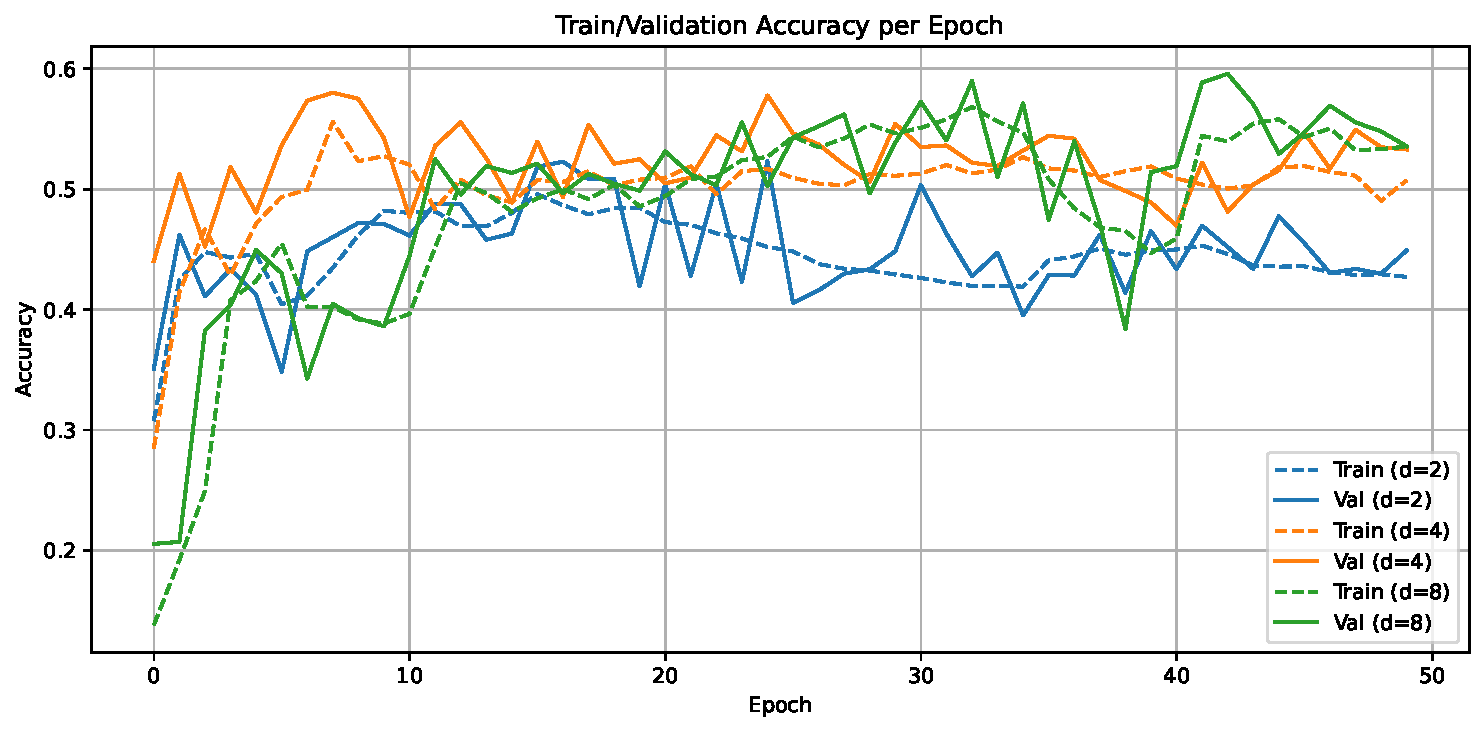
\includegraphics[width=0.85\linewidth]{figures/accuracy.pdf}
    \caption{Train and validation accuracy across 50 epochs for OSLGN models of varying depth. Depth-8 achieves the highest validation accuracy, but depth-4 shows more stable convergence.}
    \label{fig:accuracy}
\end{figure}

\begin{figure}[H]
    \centering
    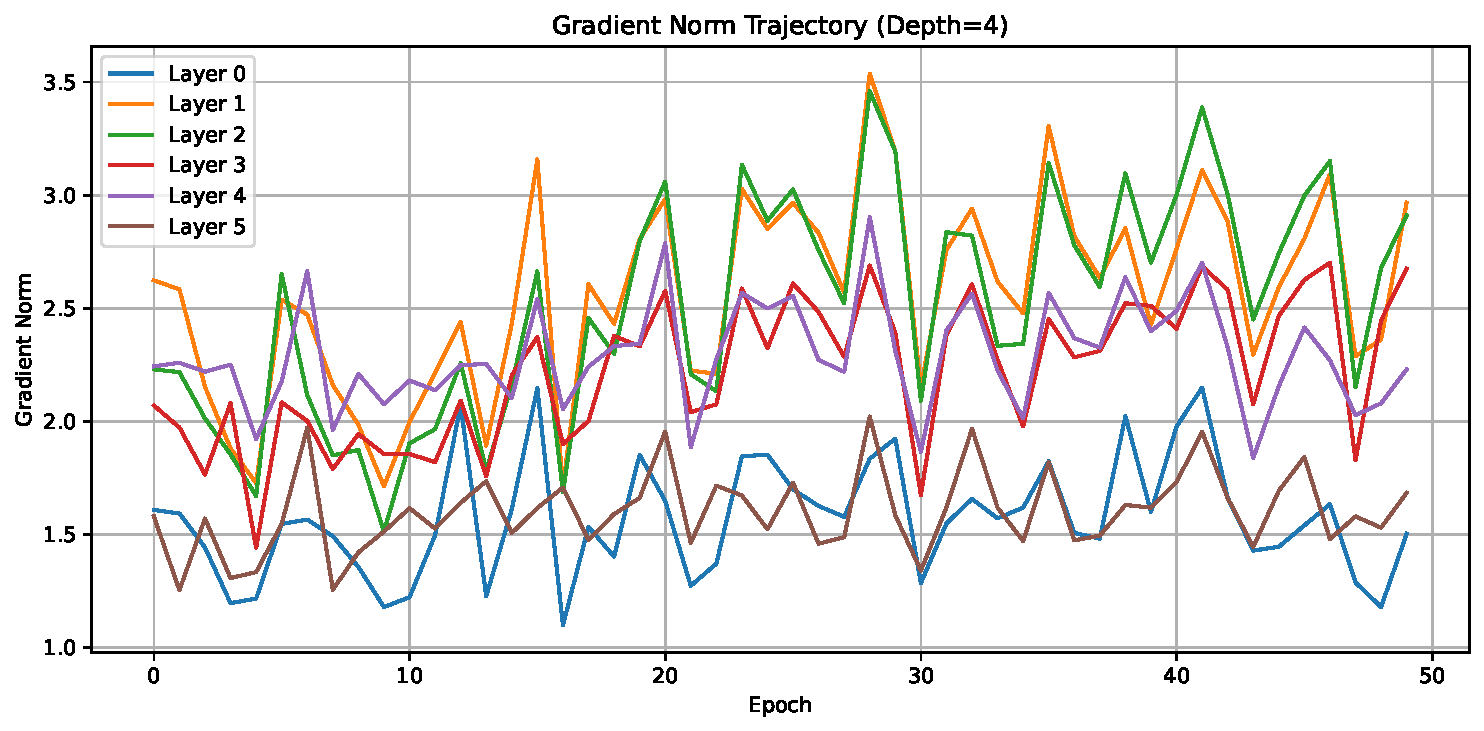
\includegraphics[width=0.45\linewidth]{figures/gradnorm_lineplot_depth4.pdf}
    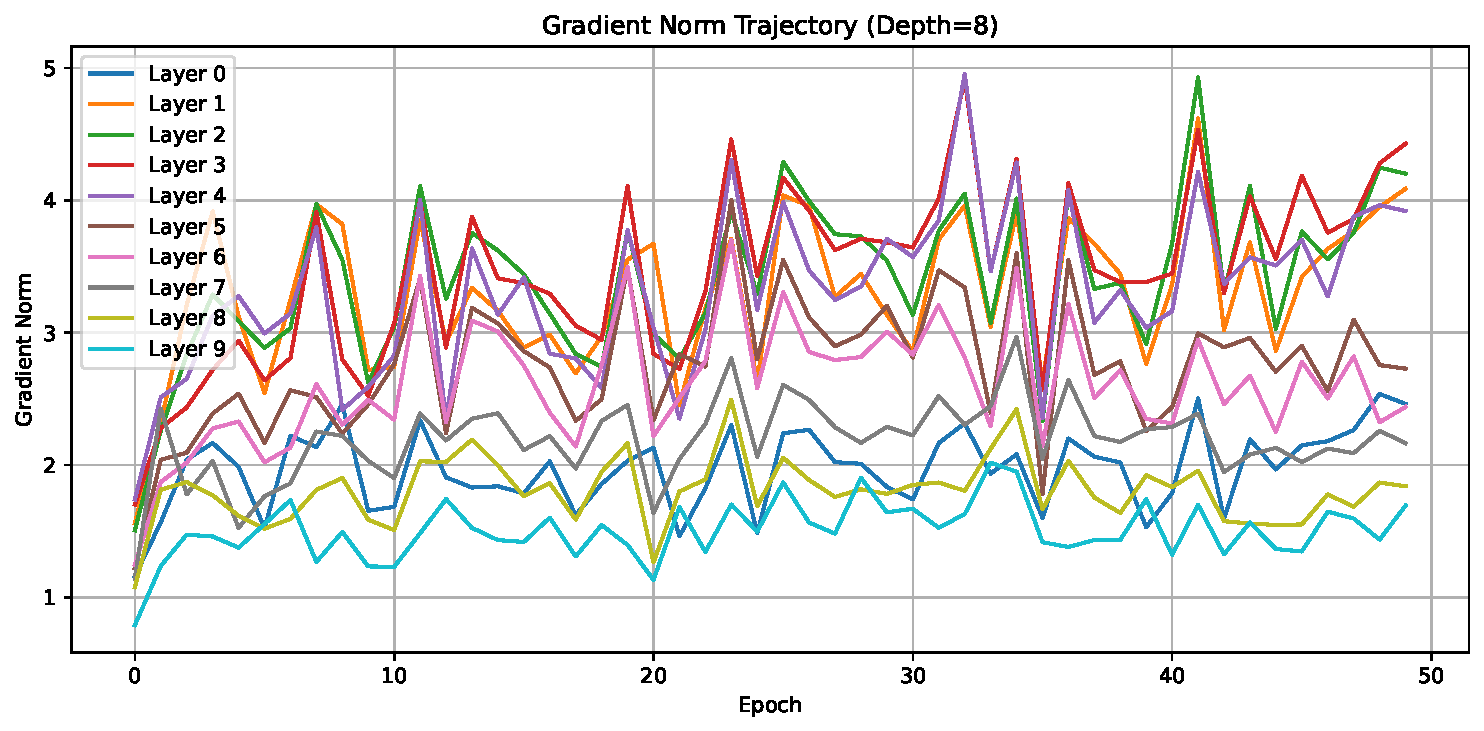
\includegraphics[width=0.45\linewidth]{figures/gradnorm_lineplot_depth8.pdf}
    \caption{Gradient norm per layer in depth-4(left) and depth-8(right) model. Optimization of depth 8 is less stable, and layer-wise imbalance is more prominent.}
    \label{fig:gradnorm_line_depth4}
\end{figure}

Figure~\ref{fig:gradnorm_line_depth4} show per-layer gradient norms for depth-4 and depth-8 models, respectively. 
We observe no gradient vanishing across layers; however, the depth-8 model exhibits more pronounced fluctuations and greater disparity between layers, suggesting optimization imbalance in deeper compositions.

Unlike conventional architectures, OSLGN does not employ normalization layers or residual connections, as these mechanisms interfere with the discrete and symbolic structure of binary logic gates. 
This design choice preserves the model’s logic circuit equivalence, but it also introduces training challenges, particularly in deeper networks.

Our implementation\footnote{\url{https://colab.research.google.com/drive/1PZhAzfH9bh_2cVn3s_Clmgkj0ezVr3Jw}} is publicly available and supports configurable depth, logging, and visualization, allowing researchers to explore the scalability of logic-based neural circuits further.
